\documentclass[a4paper, 12pt]{article}
\usepackage[T2A]{fontenc}
\usepackage[utf8]{inputenc}
\usepackage[english,russian]{babel}
\usepackage{amsmath, amsfonts, amssymb, amsthm, mathtools, misccorr, indentfirst, multirow}
\usepackage{wrapfig}
\usepackage{graphicx}
\usepackage{subfig}
\usepackage{adjustbox}
\usepackage{pgfplots}

\usepackage{geometry}
\geometry{top=20mm}
\geometry{bottom=20mm}
\geometry{left=20mm}
\geometry{right=20mm}
\newcommand{\angstrom}{\textup{\AA}}
\newcommand{\norm}[1]{\left\lVert#1\right\rVert}

\title{Вторая контрольная работа по вычислительной математике\\
Вариант №37}
\author{Нехаев Александр, гр. 654}
\date{\today}
\begin{document}
	\maketitle
	\pagenumbering{arabic}
	\section*{Задача №1}
	\subsection*{Условие}
	Сформулировать теорему о сходимости итерационного метода Ньютона $f(x)=0$. Показать, что при выполнении условий теоремы о сходимости метода Ньютона для скалярного уравнения $f(x)=0$ последовательность приближений 
\begin{equation*}
\left\lbrace x_n:x_n=x_{n-1}-f\left(x_{n-1}\right)/f'\left(x_{n-1}\right)\right\rbrace^\infty_{n=1}
\end{equation*}	
является ограниченной либо снизу, либо сверху.
	\subsection*{Решение}
	\paragraph{Теорема}Если $f(a)f(b)<0$, ($[a,b]$ -- отрезок локализации) причем $f_x',f_{xx}''$ непрерывные и знакопостоянные на $[a,b]$ в области локализации корня $x^*$, то исходя из начального приближения $x_0$, удовлетворяющего неравенству $f(x_0)f_{xx}''(x_0)>0$ можно получить по формуле итерационного метода Ньютона $x_{n+1}=x_n-\frac{f(x_n)}{f'_x(x_n)},\ n=0,1,2,...$, единственный корень уравнения $f(x)=0$ с любой степенью точности.
	\paragraph{Доказательство}Рассмотрим только случай $f'_x,f_{xx}''>0$. Также предположим, что $x^*<x_0$ (тогда выполнено $f(x_0)f''_{xx}(x_0)>0$). Докажем, что $\{x_n\}$ ограничена снизу.\par
	Рассмотрим значение $f(x^*)$. Оно равно 0. Разложим функцию в ряд Тейлора:
	\begin{equation*}
		f(x^*)=0=f(x_n)+f_x'(x_n)(x^*-x_n)+\frac{f_{xx}''(\xi)(x^*-x_n)^2}{2},\quad\xi\in[a,b]
	\end{equation*}
	
	Далее запишем формулу метода Ньютона в виде
	\begin{equation*}
		0=f(x_n)=f'_x(x_n)(x_{n-1}-x_n)
	\end{equation*}
	
	После простого преобразования легко видеть:
	\begin{equation}
		\label{eq:1}
		f_x'(x_n)(x^*-x_{n+1})+\frac{f''_{xx}(\xi)(x^*-x_n)^2}{2}=0
	\end{equation}
	В области локализации $f''_{xx}>0\ \Rightarrow$ все второе слагаемое левой части (\ref{eq:1}) положительно.
	
	Следовательно:
	\begin{equation*}
		f'_x(x_n)(x^*-x_{n+1})<0\rightarrow x^*-x_{n+1}<0\Rightarrow x^*<x_{n+1}
	\end{equation*}
	значит последовательность ограничена снизу.
	
	Аналогично доказывается ограниченность сверху.
	\section*{Задача №2}
	\subsection*{Условие}
	Для решения задачи Коши (a) предложена разностная схема (б). Исследовать разностную задачу (б) на аппроксимацию и определить порядок сходимости её решения к следу решения дифференциальной задачи (а) при $h=1/L\rightarrow 0$.
	\begin{alignat*}{2}
		& \begin{aligned}
		\text{a)}\ \begin{cases}
		\frac{d^2y}{dx^2}=a,\quad a=\mbox{const}\\
		y(0)=0,\quad y'_x(0)=0,\quad x\in [0,1]
		\end{cases}\\
		\end{aligned}
		& \hskip 5em &
  		\begin{aligned}
  		\text{б)}\ \begin{cases}
  		\frac{y_{l+1}-2y_l+y_{l-1}}{h^2}=a,\quad l=\overline{1,L-1}\\
  		y_0=0,\quad(-y_2+4y_1-3y_0)/2h=0
  		\end{cases}\\
  		\end{aligned}
	\end{alignat*}
	\subsection*{Решение}
	Вектор невязки:
	\begin{equation*}
		\delta f^{(h)}=\begin{cases}
		\frac{[y]_{l+1}-2[y]_l+[y]_{l-1}}{h^2}-a\\
		[y]_0-0\\
		\frac{-[y]_{2}-4[y]_1-3[y]_{0}}{2h}-0
		\end{cases}
	\end{equation*}
	
	Ряды:
	\begin{equation*}
	[y]_{l\pm 1}=[y]_l\pm[y'_x]_lh+[y''_x]_l\frac{h^2}{2}\pm[y'''_x]_l\frac{h^3}{6}+[y''''_x]_l\frac{h^4}{24}+o(h^3)
	\end{equation*}
	\begin{equation*}
	[y]_1=[y]_0+[y'_x]_0 h+[y''_x]_0 \frac{h^2}{2}+[y'''_x]_0\frac{h^3}{6}+o(h^4)\\
	\end{equation*}
	\begin{equation*}
	[y]_2=[y]_0+[y'_x]_0 2h+[y''_x]_0 \frac{4h^2}{2}+[y'''_x]_0\frac{8h^3}{6}+o(h^4)\\
	\end{equation*}
	
	Подставив, получим:
	\begin{equation*}
		\delta f^{(h)}=\begin{cases}
		[y''_x]_l-a+[y''''_x]\cdot\frac{h^2}{12}+o(h^3)\\
		0\\
		[y'_x]_0+[y_x''']_0\cdot\frac{h^3}{2}+o(h^4)
		\end{cases}=
		\begin{cases}
		ch^2\\
		0\\
		ch^3
		\end{cases}
	\end{equation*}
	\begin{equation*}
		\norm{\delta f^{(h)}}=\max_l\left(|\delta f_l|\right)\leqslant ch^2
	\end{equation*}
	2-й порядок аппроксимации
	
	Сходимость:\\
	Решим ЗК:
	\begin{equation*}
	y(x)=\frac{ax^2}{2}
	\end{equation*}
	След:
	\begin{equation*}
	[y]_h=\left\lbrace[y]_l=\frac{al^2h^2}{2},\ l\in\overline{0;L},\ Lh=1\right\rbrace
	\end{equation*}
	Система уравненийй:
	\begin{equation*}
	\begin{cases}
	y_0=1\\
	-y_2+4y_1-3y_0=0\\
	y_{l+1}-2y_l+y_{l-1}=ah^2
	\end{cases}
	\end{equation*}
	Характеристические уравнения:
	\begin{equation*}
	q^{l+1}-2q^l+q^{l-1}=0
	\end{equation*}
	\begin{equation*}
	q^{l-1}(q^2-2q+1)=0\Rightarrow q=1\text{ кр. } 2
	\end{equation*}
	\begin{equation*}
	y_{l_{oy}}=C_1+C_2 l
	\end{equation*}
	Ищем частные решения в виде $y_{\text{чр}}=Al^2$:
	\begin{equation*}
	A(l+1)^2-2Al^2+A(l-1)^2=ah^2
	\end{equation*}
	\begin{equation*}
	l(A-2A+A)+l(2A-2A)+(A+A)=ah^2
	\end{equation*}
	\begin{equation*}
	A=\frac{ah^2}{2}
	\end{equation*}
	\begin{equation*}
	y_l=C_1+C_2l+\frac{ah^2}{2}l^2
	\end{equation*}
	Из начальных условий:
	$y_0=0\Rightarrow C_1=0$\\
	$-y_2+4y_1-3y_0=0\Rightarrow-(0+2C_2+2ah^2)+4(0+C_2+\frac{ah^2}{2})-3=0$\\
	$2C_2=0\Rightarrow C_2=0$\\
	$y_l=0+\frac{ah^2}{2}l^2$\\
	Разность: $\norm{[y]_h-y^{(h)}}=\max_l\left(\left|\frac{a}{2}h^2l^2-0-\frac{a}{2}h^2l^2\right|\right)$\\
	\begin{equation*}
		\left|\frac{a}{2}h^2l^2-0-\frac{a}{2}h^2l^2\right|=0
	\end{equation*}
	Бесконечный порядок сходимости.
	\section*{Задача №3}
	\subsection*{Условие}
	Построить кубический сплайн для таблично заданной функции и её первой производной.
	\begin{table}[h]
		\centering
		\begin{tabular}{|c|c|c|c|}
		\hline
		$x$ & -1 & 0 & 1\\
		\hline
		$y(x)$ & -2 & 1 & 1\\
		\hline
		$y'_x(x)$ & 2 & 3/2 & 1\\
		\hline		
		\end{tabular}
	\end{table}
	\subsection*{Решение}
	Общий вид функций кубического сплайна:
	\begin{equation*}
	\begin{cases}
	S_1(x)=a_3x^3+a_2x^2+a_1x+a_0\\
	S_2(x)=b_3x^3+b_2x^2+b_1x+b_0
	\end{cases}
	\end{equation*}
	Применим условия из таблицы к этим уравнениям:
	\begin{equation*}
	\begin{cases}
	S_1(-1)=-2\\
	S_1'(-1)=2\\
	S_1(0)=1\\
	S_1'(0)=3/2
	\end{cases}\Leftrightarrow
	\begin{cases}
	a_0-a_1+a_2-a_3=-2\\
	a_1-2a_2+3a_3=2\\
	a_0=1\\
	a_1=3/2
	\end{cases}\Leftrightarrow
	\begin{cases}
	a_0=1\\
	a_1=3/2\\
	a_2=-4\\
	a_3=-5/2
	\end{cases}
	\end{equation*}
	\begin{equation*}
	\begin{cases}
	S_2(0)=1\\
	S_2'(0)=3/2\\
	S_2(1)=1\\
	S_2'(1)=1
	\end{cases}\Leftrightarrow
	\begin{cases}
	b_0=1\\
	b_1=3/2\\
	b_0+b_1+b_2+b_3=1\\
	b_1+2b_2+3b_3=1
	\end{cases}\Leftrightarrow
	\begin{cases}
	b_0=1\\
	b_1=3/2\\
	a_2=4\\
	a_3=5/2
	\end{cases}
	\end{equation*}
	Итоговый ответ:
	\begin{equation*}
	\begin{cases}
	S_1(x)=1+\frac{3x}{2}-4x^2-\frac{5x^3}{2}\\
	S_1(x)=1+\frac{3x}{2}+4x^2+\frac{5x^3}{2}
	\end{cases}
	\end{equation*}
	\begin{figure}[h]
		\centering
		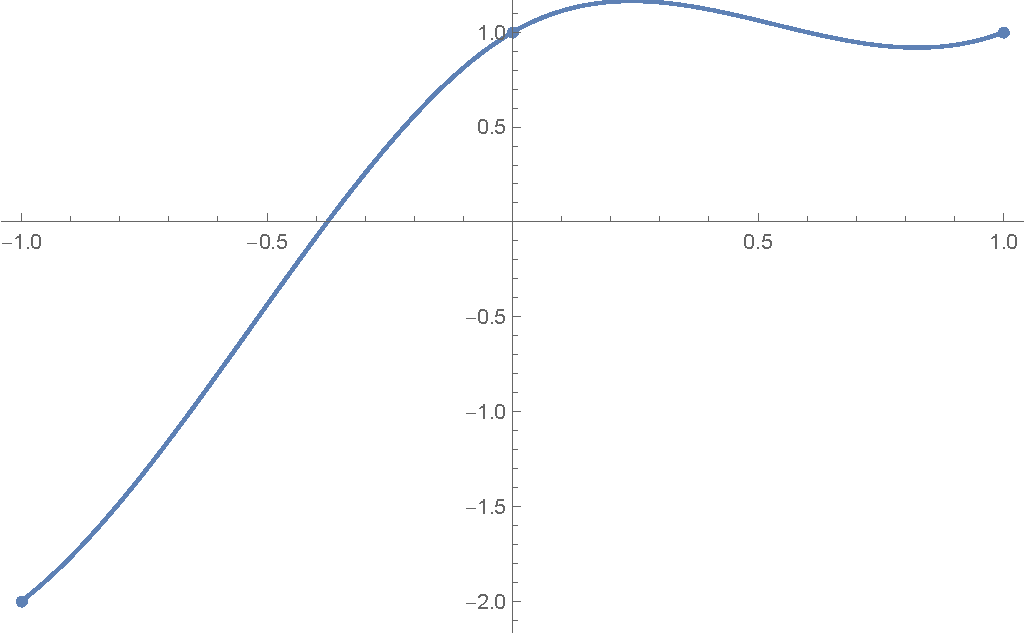
\includegraphics[scale=0.5]{spline}
		\caption{Полученный сплайн}
	\end{figure}
	\section*{Задача №4}
	\subsection*{Условие}
	Написать итерационную формулу метода Ньютона для решения системы нелинейных уравнений
	\begin{equation*}
	\begin{cases}
	xy=1\\
	\sin^2x+\sin^2y=1
	\end{cases}
	\end{equation*}
	\subsection*{Решение}
	В данном случае $f_1(x,y)=xy-1$, $f_2(x,y)=\sin^2x+\sin^2y-1$, $\frac{\partial f_1}{\partial x}=y$, $\frac{\partial f_1}{\partial y}=x$, $\frac{\partial f_2}{\partial x}=2\sin x\cos x$, $\frac{\partial f_2}{\partial y}=2\sin y\cos y$. Таким образом,
	\begin{equation*}
	\frac{\partial \vec{F}}{\partial\vec{\xi}}=\left(\begin{matrix}
	y & x\\
	2\cos x\sin x & 2\cos y\sin y
	\end{matrix}\right),\left[\frac{\partial\vec{F}}{\partial\vec{\xi}}\right]^{-1}=\frac{1}{2y\cos y\sin y-2x\cos x\sin x}\left(\begin{matrix}
	2\cos y\sin y & -x\\
	-2\cos x\sin x & y
	\end{matrix}\right),
	\end{equation*}
	где использованы обозначения $\vec{\xi}=\left(\begin{matrix}
	x\\
	y
	\end{matrix}\right)$, $\vec{F}\left(\vec{\xi}\right)=\left(\begin{matrix}
	f_1(x,y)\\
	f_2(x,y)
	\end{matrix}\right)$. В итоге получаем
	\begin{equation*}
		x_{n+1}=x_n-\frac{2(x_ny_n-1)\sin y_n\cos y_n-(\sin^2x_n+\sin^2y_n-1)x_n}{2y_n\cos y_n\sin y_n-2x_n\cos x_n\sin x_n},
	\end{equation*}
	\begin{equation*}
		y_{n+1}=y_n-\frac{y_n(\sin^2x_n+\sin^2y_n-1)-2(x_ny_n-1)\cos x_n\sin x_n}{2y_n\cos y_n\sin y_n-2x_n\cos x_n\sin x_n}.
	\end{equation*}
	\section*{Задача №5}
	\subsection*{Условие}
	При каких значениях параметра $\tau$ метод $\vec{x}_{n+1}=(E=\tau A)\vec{x}_n+\tau\vec{b},\ n=0,1,...$ решения $A\overline{x}=\overline{b}$ сходится при произвольном приближении $\overline{x}_0$ в случае $A=\left(
	\begin{matrix}
	4 & 5\\
	6 & 7
	\end{matrix}
	\right)$; $\vec{b}=\left(
	\begin{matrix}
	6\\
	8
	\end{matrix}
	\right)$.
	\subsection*{Решение}
	$\text{det}\left|A-\lambda E\right|=(4-\lambda)(7-\lambda)-30=28-4\lambda-7\lambda+\lambda^2-30=\lambda^2-11\lambda-2$.\\
	$\lambda_1=\frac{1}{2}(11-\sqrt{129}),\quad\lambda_2=\frac{1}{2}(11+\sqrt{129})$.
	\begin{equation*}
	\begin{cases}
	|1-\lambda_1\tau|<1\\
	|1-\lambda_2\tau|<1
	\end{cases}
	\end{equation*}
	Нет пересечений $\Rightarrow$ ни при каком.
\end{document}